%!TEX root = ../dissertation.tex
\chapter{Sviluppo}
In questa sezione, verranno elencate e introdotte le tecnologie che sono state utilizzate nel progetto di stage.
\section{Tecnologie}
\subsection{Google Cloud}
Il principale servizio utilizzato durante il progetto è stato Google Cloud, in esso troviamo una moltitudine di strumenti utili allo sviluppo, all'esecuzione e all'interazione di progetti riguardanti Big Data e Intelligenza Artificiale. Inoltre, importante risulta la possibilità di consultare, manipolare e presentare i dati.
Il progetto Google Cloud (anche detto Google Cloude Platform), viene lanciato nel 2008 con uno dei suoi servizi di punta ancora oggi  \gls{App Engine}. Nell'arco degli anni sia il bacino di utenti, sia i servizi offerti sono via via aumentati. Oggigiorno i suoi clienti \cite{clienti} sono molti, tra cui grandi aziende, e le funzionalità di spicco sono molteplici, i campi di maggiore interesse riguardano strumenti di Compute, Storage \& Databases, Big Data, Cloud AI e IoT.
Per quanto riguarda l'esperienza personale, ho trovato Google Cloud un buon servizio, con dei problemi da risolvere sulla completezza della documentazioni e a volte con grafiche da migliorare, ma comunque un ottimo compromesso tra qualità e prezzo.
Il resto della sezione introduce il prodotti e i servizi GCP utilizzati durante lo stage.
\begin{figure}
	\centering
	
\includegraphics[scale=0.3]{figures/google-cloud-platform}
	\caption[Logo Google Cloud Platform.]{Logo Google Cloud Platform.
		\label{fig:logoGCP}}
\end{figure}	
\subsubsection{Google Cloud Storage}
Lanciato nel 2010, Google Cloud Storage \cite{GoogleCloudStorage} è il servizio di hosting dei file della piattaforma. All'interno ogni utente può scegliere in che modalità salvare i dati (zona del mondo, carico di lavoro e frequenza d'accesso), così da trovare la soluzione maggiormente adatta ai propri bisogni.
I suoi punti di forza sono:
\begin{itemize}
	\item Interoperabilità: possibilità di interfacciarsi con strumenti e servizi di aziende terze (come Amazon S3);
	\item Consistenza: tutte le operazioni sono svolte secondo il principio di \gls{atomicità};
	\item Controllo di accesso: possibilità di definire l'accesso ad un singolo oggetto o \gls{bucket} a seconda della categoria di appartenenza degli utenti;
	\item Resumable Uploads: in caso di fallimento di un upload, questo può essere continuato/ricominciato.
\end{itemize}

Per quanto riguarda l'esperienza d'utilizzo, si è rivelato un ottimo servizio di storage, l'abilitazione di un'unica API rende disponibile l'intero pacchetto di funzionalità e ciò l'ho trovato molto comodo.
\subsubsection{Google Cloud BigQuery}
Servizio lanciato insieme a Google Cloud Storage nel 2010, Google Cloud BigQuery \cite{GoogleCloudBigQuery}, è lo strumento che permette di interagire e analizzare grandi moli da dati, definito come un \gls{data warehouse}. All'interno di GCP, vi è un'apposita interfaccia utente per utilizzarlo. Si basa su tabelle codificate in formato JSON e sulla quale vengono processate query in standard SQL \cite{standardSQL} tramite avanzati algortmi di \gls{MapReduce}.
\\I principali punti di forza sono:
\begin{itemize}
	\item La piattaforma rende disponibile la creazione e distruzione di tabelle basati su schemi JSON, inoltre rende disponibile l'import e l'export di dati in formati come CSV e JSON;
	\item La semplicità del linguaggio SQL con scalabilità e prestazioni che solo i servizi cloud riescono a dare;
	\item Un'ottima integrazione con servizi e API esterni, per la raccolta e l'utilizzo dei dati;
	\item Possibilità di garantire l'accesso ad uno o più categorie di utenti;
	\item Possibilità di interagire con strumenti di Machine Learning nativi di Google e non (come TensorFlow).
\end{itemize}

L'opinione del team di sviluppo riguardo lo strumento è molto positiva sopratutto grazie alla scalabilità automatica che rende semplice e veloce l'utilizzo delle query su grandi moli di dati, un possibile punto di debolezza può essere trovato nell'utilizzo in sola lettura dei dati esistenti, quindi non vi è la possibilità di modifica dei record se non un nuovo inserimento.
\subsubsection{Google Cloud Dataflow}
Rilasciato al pubblico nel 2015, Google Cloud Dataflow \cite{GoogleCloudDataflow} è lo strumento che permette di processare pipeline per l'integrazione, la preparazione e l'analisi di grandi quantità di dati.
Il modello di pipeline consigliato è quello di Apache Beam che vedremo in seguito.
\\ Tra i maggiori punti di forza troviamo:
\begin{itemize}
	\item Creazione di pipeline secondo modelli già esistenti o personalizzati dall'utente;
	\item Composizione di pipeline, e quindi job specifici, direttamente da codice;
	\item Possibilità di utilizzo di dati da molteplici fonti, non solo da strumenti Google;
	\item Ottima scalabilità interna in base agli effettivi bisogni del lavoro in esecuzione;
	\item Buona granularità della specificazione dei parametri di esecuzione\cite{parametridiesecuzione} della pipeline;
	\item Visualizzazione grafica della pipeline (Possibile immagine?????). 
\end{itemize}
Per quanto concerne l'utilizzo di questo prodotto, il team si esprime con un giudizio più che positivo dato anche la grande quantità di documentazione disponibile.
\subsubsection{Google Data Studio}
Lanciato nel 2016, \href{https://datastudio.google.com/overview}{Google Data Studio} è lo strumento di creazione e visualizzazione dei dati attraverso report e dashboard. L'idea che sta alla base di questo tool è la condivisione dei dati che sono presenti all'interno di GCP attraverso tabelle e grafici.
\\ I maggiori vantaggi nell'utilizzarlo sono:
\begin{itemize}
	\item Accesso ai dati personali di GCP;
	\item Possibilità di integrare i dati fra di loro con query standard SQL;
	\item Condivisione a gruppi di utenti. 
\end{itemize}

Durante l'esperienza lo strumento si è rivelato molto acerbo nelle sue funzionalità e nell'utilizzo, oltre a dover attendere troppo tempo per il caricamento di dati e grafici. L'idea alla base è ottima, dato che vi è la possibilità di utilizzare i dati all'interno di GCP anche in continuo aggiornamento, d'altro canto la documentazione e l'interfaccia utente non rendono semplice quanto potrebbero la creazione di un report aziendale da presentare al cliente.
\subsubsection{Google Cloud Function}
Rilasciato in beta nel 2017, \href{https://cloud.google.com/functions/}{Google Cloud Functions} è il perfetto intermediario tra gli eventi che vengono scaturiti nel cloud e l'invocazione di servizi API. Le origini degli eventi supportati sono:
\begin{itemize}
	\item Cloud Pub/Sub;
	\item Cloud Storage;
	\item HTTP;
	\item Stackdriver Logging;
	\item Firebase. 
\end{itemize}
Inoltre, per ogni tipologia di evento vi sono ulteriori specificazioni che non verranno trattate tutte in modo estensivo in questo elaborato.
\\
Per quanto concerne l'utilizzo svolto durante il progetto, il team ritiene questo strumento valido e con ottime potenzialità e margini di miglioramento. Uno svantaggio molto importante da sottolineare è la scarsa documentazioni presente nelle fonti ufficiali.
\subsubsection{Google Cloud Composer}
\url{https://cloud.google.com/composer/?hl=it}
\subsection{Apache NiFi}
\begin{quotation}
An easy to use, powerful, and reliable system to process and distribute data.
	\qauthor{NiFi Creator}
\end{quotation}
La descrizione che viene data nella documentazione di \href{https://nifi.apache.org/docs/nifi-docs/html/getting-started.html}{NiFi} riassume alla perferzione le caratteristiche di questo strumento e ciò che ci permette di fare.
\\Innanzitutto, le sue funzioni sono proprio quelle di automatizzare lo "scorrere" del flusso dati all'interno del sistema in cui viene utilizzato. Le funzionalità sono molteplici e ben rodate, vanno dal semplice spostamento dei file, al filtraggio, composizione e conversione in diversi formati. La documentazione è molto esauriente, spiegando anche più del necessario tutti i passaggi da seguire per utilizzare un determinato componente. La semplicità e l'intuitività nel costruire il flusso di dati, rendono l'esperienza utente decisamente piacevole, anche grazie all'interfaccia grafica semplice e intuitiva. Altro punto a favore è l'affidabilità del prodotto e la grande quantità di componenti disponibili orientati alla sicurezza, così da rendere il passaggio di informazioni in più sicuro possibile.
\begin{figure}[h!]
	\centering
	\includegraphics[scale=0.1]{figures/apache-nifi-logo}
	\caption[Logo Google Cloud Platform.]{Logo Google Cloud Platform
		\label{fig:logoGCP}}
\end{figure}	
\subsection{Apache Beam}
\href{http://www.vldb.org/pvldb/vol8/p1792-Akidau.pdf}{Apache Beam} è un implementazione del \href{https://ai.google/research/pubs/pub43864}{modello Dataflow}, esso infatti fissa come definire ed eseguire pipeline sui dati di tipo \gls{ETL}, batch e streaming continui. Questo progetto nasce dopo il rilascio di un \gls{SDK} contenente un implementazione del modello Dataflow da parte di Google nel 2014, nel 2016 Google decise di concedere il core del proprio SDK per costituire il progetto \gls{OpenSource} Apache Beam.
\\ I concetti alla base di questa implementazione, e quindi del modello Dataflow, possono essere riassunti nel cercare un modello il quale riesca a definire ed eseguire pipeline di tipo batch e streaming allo stesso tempo, senza dover differenziare le pipeline come nel modello \href{https://en.wikipedia.org/wiki/Lambda_architecture}{Lambda architecture}.
\\ Un tipico utilizzo di una pipeline può essere il seguente:
\begin{figure}[h!]
	\centering
	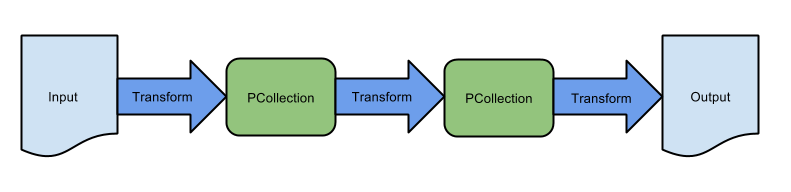
\includegraphics[scale=0.5]{figures/design-your-pipeline-linear}
	\caption[Esempio utilizzo Apache Beam. ]{Esempio utilizzo Apache Beam.
		\label{fig:logoGCP}}
\end{figure}	
\begin{itemize}
	\item Creazione della Pipeline;
	\item Creazione di una PCollection da dei dati di input;
	\item Applicazione di PTrasforms sulla PCollection;
	\item Scrittura dei dati all'interno di un file.
\end{itemize}
Le azioni di maggiore interesse stanno nelle PTrasforms, infatti rende possibile processare ogni singolo elemento delle PCollection, effettuare raggruppamenti per uno o più elementi, unire  e partizionare le PCollections.
La documetazione a disposizione è decisamente idonea e precisa rispetto alla potenzialità di utilizzo. Inoltre, essendo un progetto OpenSource vi è la possibilità di collaborare al continuo sviluppo, e quindi al successo, che questa tecnologia sta avendo.
\subsection{Apache AirFlow}
\href{https://airflow.apache.org/}{Apache AirFlow} è una piattaforma per creare, schedulare e monitorare \gls{workflows}. Airflow, inoltre, cerca la soluzione più performante per l'esecuzione dei task, creando un Grafo Aciclico Diretto (meglio conosciuto come "\gls{DAGs}" cioe " Directed Acyclic Graphs") in modo da riconoscere le dipendenze tra i compiti stessi ed eseguire i task con meno dipendenze.
La scelta di utilizzare questa tecnologia è stata presa sia per la già precedente esperienza aziendale con essa, sia perché completamente compatibile e già installata all'interno di Google Cloud Composer. Data la sua notevole compatibilità ci ha permesso di soddisfare un requisito del cliente riguardante l'ingestion in tempo reale dei dati inviati.
\subsection{Docker}
\subsection{Apache Spark}
\subsubsection{Apache Spark MlLib}
\section{Integrazione}
\begin{figure}[h!]
	\centering
	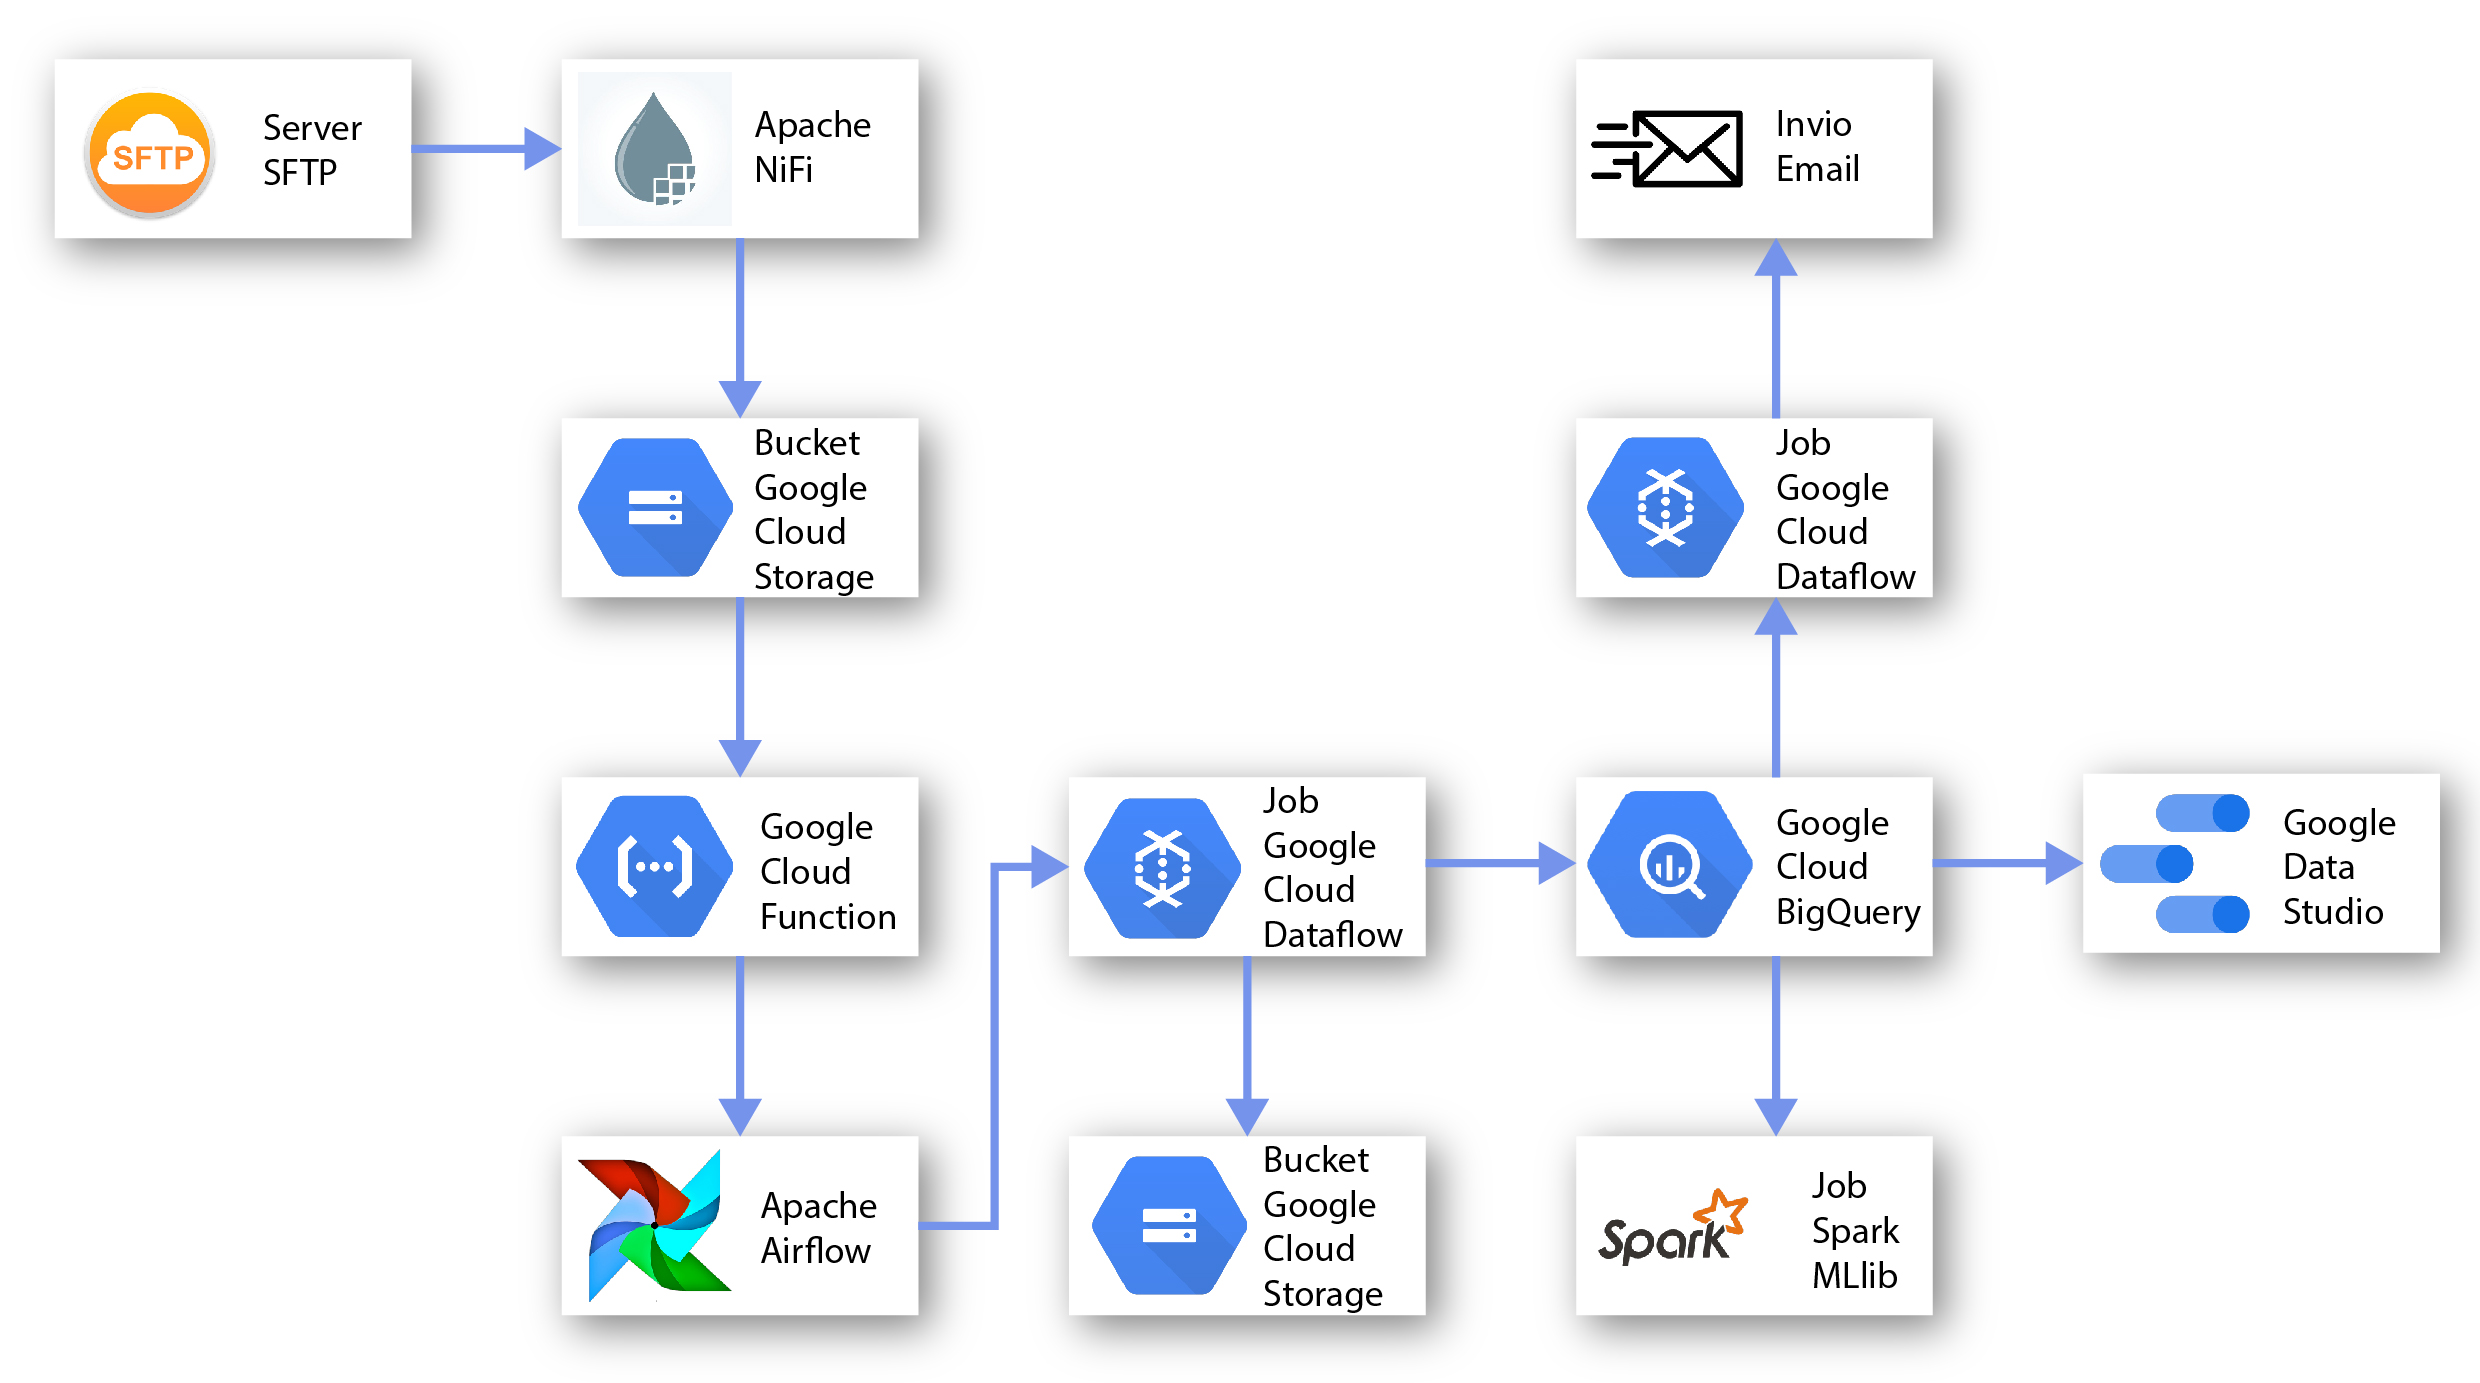
\includegraphics[scale=0.7]{figures/Schema_complessivo}
	\caption[Workflow progetto	.]{Workflow progetto.
		\label{fig:logoGCP}}
\end{figure}	
L'integrazione delle tecnologie elencate alla sezione 4.1, ha portato a stabilire un vero e proprio ciclo di vita del dato. Infatti, partendo dai file che il cliente rilascia giornalmente all'interno di un \gls{server SFTP}(1), tramite Apache NiFI (2), avveniva una prima pre elaborazione in base alla tipologia di file così da unificare il formato su cui lavorare.
\\
Questi file vengono spostati all'interno di Google Cloud Storage (3), il quale, al trasferimento di ogni file, scatena l'avvio delle Google Cloud Function (4) che di conseguenza avviano il processo di ingestion sul file appena trasferito tramite l'attivazione del file DAGs all'interno di AirFlow (5).
\\
L'ingestion è composta da alcuni job Google Cloud Dataflow (6) scritti in \gls{Python} e caratterizzati dall'utilizzo di Apache Beam (7) per la creazione delle pipeline dei dati.
Questi job, rendono i dati leggibili e consultabili. Dopodiché, vengono riportati all'interno di apposite tabelle Google Cloud BigQuery (8).
\\
Al termine di questo processo, abbiamo il definitivo passaggio da semplice dato ad effettiva informazione per cliente tramite i report e le dashborad riassuntive di Google Data Studio (9).
\\
Per concludere il processo da dato ad informazione, abbiamo costruito un sistema che, tramite Kafka (10) e quindi secondo lo schema produttore-consumatore in streaming, invia dei dati ad un algoritmo di Machine Learning sviluppato tramite Apache Spark (11)(più in particolare tramite la libreria Apache Spark MLlib) che classifica gli utenti su base settimanale, conserva le classificazioni e verifica che ogni utente non abbia cambi di classe in modo anomalo.

Come?

Durante l'esperienza lo strumento si è rilevato...